\documentclass[11pt,a4paper]{article}
\usepackage{fontspec}
\setmainfont[Path=fonts/,FontIndex=7,BoldFont=AvenirNext.ttc,BoldFeatures={FontIndex=2},ItalicFont=AvenirNext.ttc,ItalicFeatures={FontIndex=4},BoldItalicFont=AvenirNext.ttc,BoldItalicFeatures={FontIndex=3}]{AvenirNext.ttc}
\setsansfont[Path=fonts/,FontIndex=7,BoldFont=AvenirNext.ttc,BoldFeatures={FontIndex=2},ItalicFont=AvenirNext.ttc,ItalicFeatures={FontIndex=4},BoldItalicFont=AvenirNext.ttc,BoldItalicFeatures={FontIndex=3}]{AvenirNext.ttc}
\newfontfamily\heavy[Path=fonts/,FontIndex=2]{AvenirNext.ttc}
\setmonofont[Path=fonts/,BoldFont=JetBrainsMono-Bold.ttf,ItalicFont=JetBrainsMono-Italic.ttf,Contextuals=NoAlternate,Ligatures=NoCommon]{JetBrainsMono-Regular.ttf}
\usepackage{xcolor,graphicx,tikz,booktabs,tabularx,listings,amsmath}
\usetikzlibrary{arrows.meta,positioning}
\definecolor{paper}{HTML}{FFFFFF}
\definecolor{ink}{HTML}{252525}
\definecolor{teal}{HTML}{252525}
\definecolor{orange}{HTML}{777777}
\definecolor{wash}{HTML}{EAEAEA}
\definecolor{quiet}{HTML}{666666}
\definecolor{lightink}{HTML}{D0D0D0}
\definecolor{codepaper}{HTML}{F6F6F4}
\lstset{language=Python,basicstyle=\ttfamily\fontsize{9.5}{13}\selectfont\color{ink},keywordstyle=\bfseries\color{ink},commentstyle=\itshape\color{quiet},stringstyle=\color{ink},showstringspaces=false,columns=fullflexible,keepspaces=true,breaklines=true,breakatwhitespace=true,numbers=none,upquote=true,aboveskip=8pt,belowskip=6pt}
\hyphenpenalty=4000
\emergencystretch=3em
% The same two-line navigation and fine rule as the reference, without a candy motif.
\newcommand{\guideheader}[2]{\begin{tikzpicture}[remember picture,overlay]
\node[anchor=north west,inner sep=0,text width=176mm] at ([xshift=16mm,yshift=-7mm]current page.north west) {\fontsize{8.5}{10}\selectfont\color{quiet}#1};
\node[anchor=north west,inner sep=0,text width=176mm] at ([xshift=16mm,yshift=-11.5mm]current page.north west) {\heavy\fontsize{10}{12}\selectfont\color{ink}#2};
\draw[lightink,line width=.4pt] ([xshift=16mm,yshift=-17mm]current page.north west)--([xshift=192mm,yshift=-17mm]current page.north west);
\end{tikzpicture}}

\usepackage[a4paper,left=16mm,right=18mm,top=24mm,bottom=19mm,headheight=14pt]{geometry}
\usepackage{fancyhdr,enumitem,hyperref}
\hypersetup{colorlinks=true,linkcolor=teal,urlcolor=teal}
\setlength{\parindent}{0pt}
\setlength{\parskip}{7pt}
\setlist{nosep,leftmargin=1.4em}
\usepackage{needspace,colortbl}
\lstdefinestyle{numbered}{numbers=left,numberstyle=\ttfamily\fontsize{7.5}{13}\selectfont\color{lightink},numbersep=10pt,xleftmargin=24pt}
\pagestyle{fancy}\fancyhf{}
\fancyhead[C]{\guideheader{Lesson 2 · Dice Combinations and Grid Paths}{Worksheet · \nouppercase{\leftmark}}}
\fancyfoot[L]{\fontsize{8}{10}\selectfont\color{quiet}LESSON 2 / Dice Combinations and Grid Paths}
\fancyfoot[R]{\fontsize{9}{11}\selectfont\color{quiet}\thepage}
\renewcommand{\headrulewidth}{0pt}
\newcommand{\topic}[2]{\clearpage\markboth{#2}{}{\color{quiet}\fontsize{9}{12}\selectfont\textbf{#1}}\par{\heavy\fontsize{19}{23}\selectfont\raggedright #2\par}\vspace{5pt}}
\newcommand{\topicflow}[2]{\par\Needspace{20\baselineskip}\bigskip\markboth{#2}{}{\color{quiet}\fontsize{9}{12}\selectfont\textbf{#1}}\par{\heavy\fontsize{19}{23}\selectfont\raggedright #2\par}\vspace{5pt}}
\newcommand{\labeltext}[1]{{\color{teal}\textbf{#1}}\par}
\begin{document}\color{ink}\fontsize{10.5}{13}\selectfont
\thispagestyle{empty}\pagecolor{white}\null
\begin{tikzpicture}[remember picture,overlay]
\node[anchor=north west,inner sep=0,text width=174mm] at ([xshift=18mm,yshift=-22mm]current page.north west)
{\heavy\fontsize{9}{12}\selectfont ALGORITHMS\quad /\quad LESSON 02\quad /\quad PRINTER-FRIENDLY WORKSHEET};
\node[anchor=north west,inner sep=0,text width=174mm] at ([xshift=18mm,yshift=-39mm]current page.north west)
{\heavy\fontsize{43}{47}\selectfont\raggedright\spaceskip=.25em Dice and\\Grid Paths\par};
\node[anchor=north west,inner sep=0,text width=174mm] at ([xshift=18mm,yshift=-80mm]current page.north west)
{\fontsize{19}{25}\selectfont Questions, diagrams and tables.};
\node[anchor=north west,inner sep=0,text width=150mm] at ([xshift=18mm,yshift=-97mm]current page.north west)
{\fontsize{12}{16}\selectfont Try each question on paper or in the notebook.\\Use the same question IDs to check your answers.};
\node[anchor=center,inner sep=0] at ([xshift=105mm,yshift=-167mm]current page.north west)
{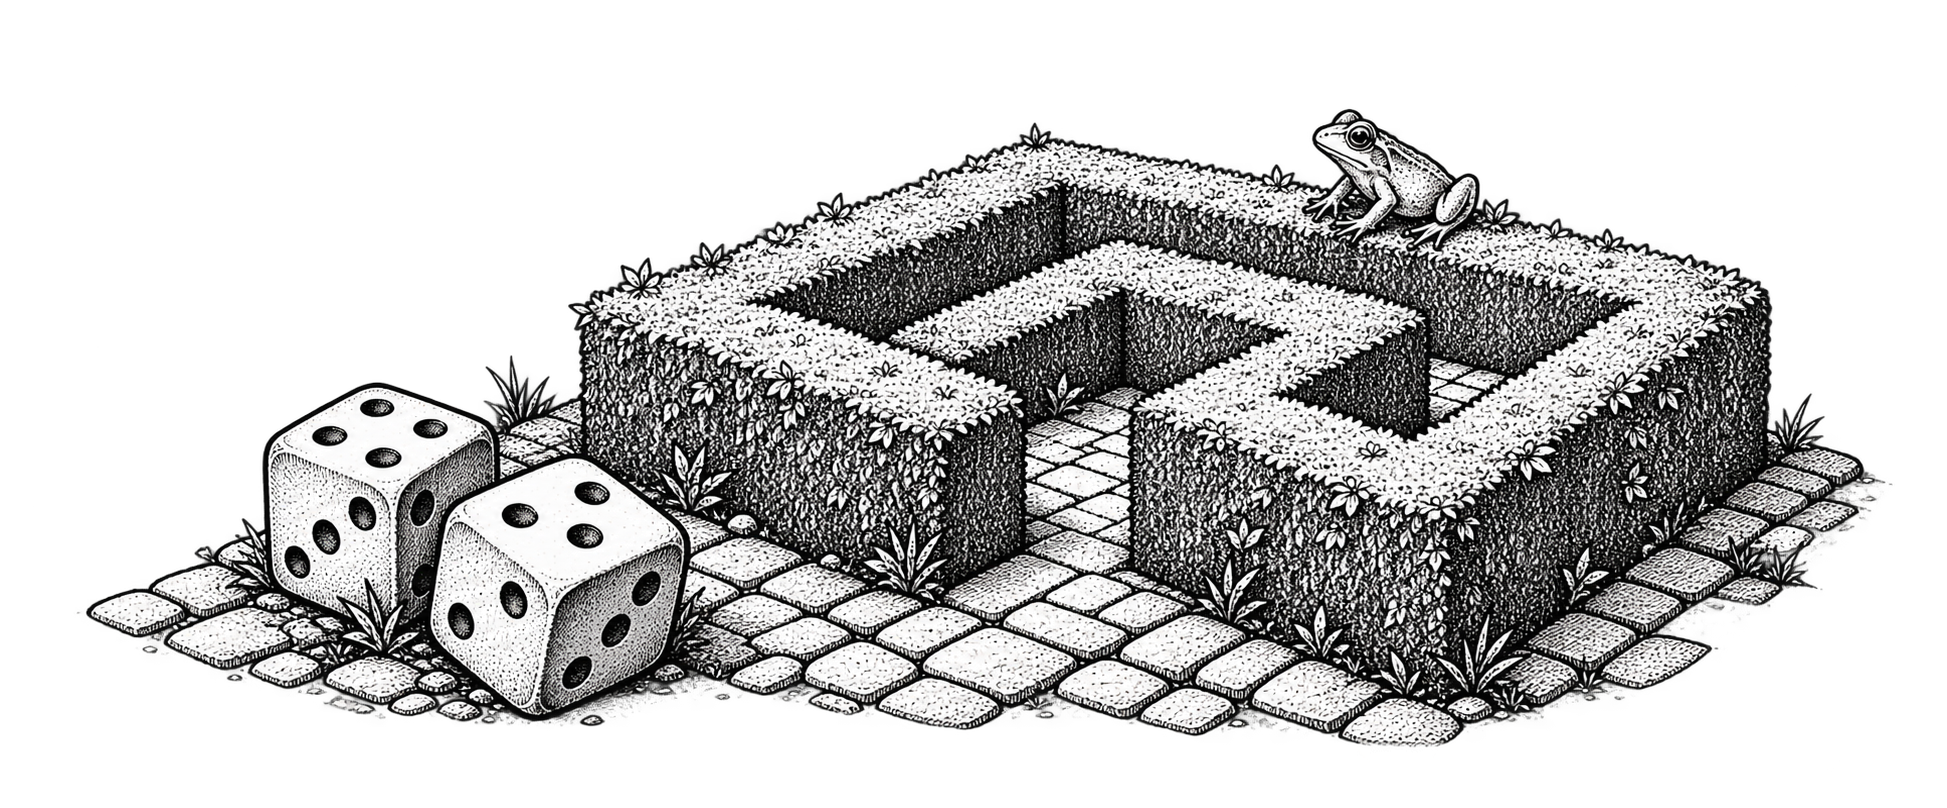
\includegraphics[width=174mm,height=94mm,keepaspectratio]{assets/cover.png}};
\node[anchor=north west,inner sep=0,text width=174mm] at ([xshift=18mm,yshift=-224mm]current page.north west)
{\fontsize{12}{16}\selectfont Understand what each step establishes\\and why it leads to the next.};
\node[anchor=west,inner sep=0] at ([xshift=18mm,yshift=-269mm]current page.north west)
{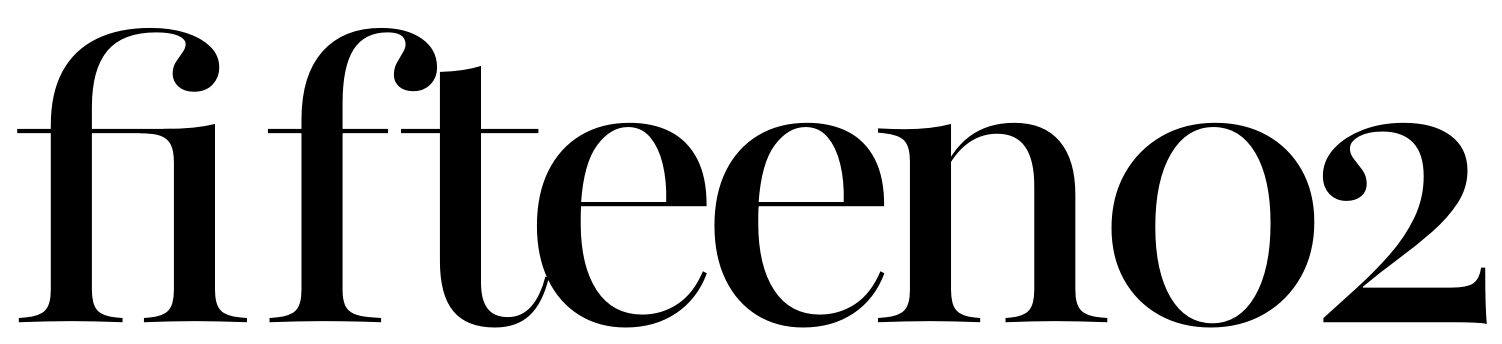
\includegraphics[width=43mm]{assets/logo.png}};
\node[anchor=east,inner sep=0] at ([xshift=192mm,yshift=-269mm]current page.north west)
{
\includegraphics[width=62mm]{assets/julians-pathfinder-monochrome.pdf}};
\node[anchor=north west,inner sep=0,text width=174mm] at ([xshift=18mm,yshift=-244mm]current page.north west) {\fontsize{11}{14}\selectfont \href{https://colab.research.google.com/github/fifteen02/julians-pathfinder/blob/main/Lesson\%202/lesson.ipynb}{\underline{Open this lesson in Google Colab}}};
\end{tikzpicture}\clearpage
\markboth{Questions}{}\raggedbottom\setlength{\parskip}{4pt}
{\heavy\fontsize{16}{20}\selectfont Lesson 2 / Dice Combinations and Grid Paths\par}\medskip
\par\noindent\begin{minipage}{\linewidth}
{\heavy\fontsize{12}{15}\selectfont Dice: count ordered sequences\par}\medskip
\textbf{L2-01 / Recall: what are we storing?}\par\smallskip In staircase, what does ways[4] = 5 mean? In Frog, what does best[4] = 30 mean? Which problem adds and which takes a minimum?\par
\end{minipage}\par\vspace{4mm}
\par\noindent\begin{minipage}{\linewidth}
\textbf{L2-02 / A total of three}\par\smallskip List every ordered sequence of numbers from 1 to 6 whose sum is exactly 3. What happens to sequences containing a 4, 5 or 6?\par
\end{minipage}\par\vspace{4mm}
\par\noindent\begin{minipage}{\linewidth}
\textbf{L2-03 / Six possible last numbers}\par\smallskip Let ways[total] count ordered sequences of values 1 to 6 whose sum is that total. Explain ways[0] = 1. For target 4, group sequences by their last number and add the earlier counts. Copy your L2-02 count into total 3, then fill totals 5, 6 and 7 in the table.\par
\par\medskip \begingroup\small\setlength{\tabcolsep}{4pt}\renewcommand{\arraystretch}{1.35}\begin{tabularx}{\linewidth}{>{\raggedright\arraybackslash}l>{\raggedright\arraybackslash}X>{\raggedright\arraybackslash}X>{\raggedright\arraybackslash}X>{\raggedright\arraybackslash}X>{\raggedright\arraybackslash}X>{\raggedright\arraybackslash}X>{\raggedright\arraybackslash}X>{\raggedright\arraybackslash}X}\toprule\textbf{Total} & \textbf{0} & \textbf{1} & \textbf{2} & \textbf{3} & \textbf{4} & \textbf{5} & \textbf{6} & \textbf{7}\\\midrule
ways[total] & 1 & 1 & 2 & ? & ? & ? & ? & ?\\
\bottomrule\end{tabularx}\endgroup\par\medskip 
\end{minipage}\par\vspace{4mm}
\par\noindent\begin{minipage}{\linewidth}
\textbf{L2-04 / Dice: recursion, then caching}\par\smallskip Write dice\_slow(n) recursively to count ordered sequences of faces 1 to 6 with total n. Trace target 4. Then write dice\_cached(n), adding a cache: which input identifies a repeated question? Use the uncached version only on tiny targets. In the cached version, store counts modulo 1,000,000,007.\par
\par\smallskip{\small\textbf{Start with:}}\par\smallskip\noindent\colorbox{codepaper}{\parbox{\dimexpr\linewidth-2\fboxsep\relax}{\small\ttfamily\raggedright def dice\_slow(n):\\\hspace*{2.4em}return None  \# Replace with your answer.\\\mbox{}\\def dice\_cached(n):\\\hspace*{2.4em}def count(total):\\\hspace*{4.8em}return None  \# Your helper goes here.\\\hspace*{2.4em}return count(n)}}\par
{\small\textbf{What each function returns.}\par dice\_slow(n): the exact number of ordered dice sequences with total n.\par dice\_cached(n): the count for total n, modulo 1,000,000,007.\par count(total): the count for this total, modulo 1,000,000,007.\par }
{\small\textbf{Hints.}}\begin{itemize}\item What is the count for total 0?\item Which faces can be the last one when the remaining total is small?\item What input identifies a repeated question, and where must the saved answers live so that every call shares them?\end{itemize}
\end{minipage}\par\vspace{4mm}
\par\noindent\begin{minipage}{\linewidth}
\textbf{L2-05 / Dice: fill the totals in order}\par\smallskip Write dice\_table(n) using a loop. Store in ways[total] the count for that total, modulo 1,000,000,007. Fill totals from 1 upwards. When the loop reaches total 7, which earlier totals does it read? Add their counts and explain the result.\par
\par\smallskip{\small\textbf{Start with:}}\par\smallskip\noindent\colorbox{codepaper}{\parbox{\dimexpr\linewidth-2\fboxsep\relax}{\small\ttfamily\raggedright def dice\_table(n):\\\hspace*{2.4em}return None  \# Replace with your answer.}}\par
{\small\textbf{What each function returns.}\par dice\_table(n): the number of ordered dice sequences with total n, modulo 1,000,000,007.\par }
{\small\textbf{Hints.}}\begin{itemize}\item Which entry is known before the loop?\item For each total, which earlier totals can the last face come from?\item Where do you take the remainder so that stored numbers stay small?\end{itemize}
\end{minipage}\par\vspace{4mm}
\par\noindent\begin{minipage}{\linewidth}
\textbf{L2-06 / Why take a remainder?}\par\smallskip Modulo 7 means the remainder after division by 7. Compare (12 + 13) \% 7 with ((12 \% 7) + (13 \% 7)) \% 7. Why do both calculations give the same remainder? How does this help when dice counts become very large?\par
\end{minipage}\par\vspace{4mm}
\par\noindent\begin{minipage}{\linewidth}
\textbf{L2-07 / Your turn: three faces}\par\smallskip Write dice\_123(n) by adapting dice\_table from L2-05 to allow only faces 1, 2 and 3. First fill counts for totals 0 through 5, then write and test your code. Explain the answer for total 5.\par
\par\smallskip{\small\textbf{Start with:}}\par\smallskip\noindent\colorbox{codepaper}{\parbox{\dimexpr\linewidth-2\fboxsep\relax}{\small\ttfamily\raggedright def dice\_123(n):\\\hspace*{2.4em}return None  \# Replace with your answer.}}\par
{\small\textbf{What each function returns.}\par dice\_123(n): the number of ordered sequences of 1, 2 and 3 with total n, modulo 1,000,000,007.\par }
{\small\textbf{Hints.}}\begin{itemize}\item Which part of dice\_table depends on the faces allowed?\item Check total 4 by hand before you run the code.\end{itemize}
\par\medskip \begingroup\small\setlength{\tabcolsep}{4pt}\renewcommand{\arraystretch}{1.35}\begin{tabularx}{\linewidth}{>{\raggedright\arraybackslash}l>{\raggedright\arraybackslash}X>{\raggedright\arraybackslash}X>{\raggedright\arraybackslash}X>{\raggedright\arraybackslash}X>{\raggedright\arraybackslash}X>{\raggedright\arraybackslash}X}\toprule\textbf{Total} & \textbf{0} & \textbf{1} & \textbf{2} & \textbf{3} & \textbf{4} & \textbf{5}\\\midrule
ways[total] & 1 &  &  &  &  & \\
\bottomrule\end{tabularx}\endgroup\par\medskip 
\end{minipage}\par\vspace{4mm}
\par\noindent\begin{minipage}{\linewidth}
{\heavy\fontsize{12}{15}\selectfont Optional: reuse six counts\par}\medskip
\textbf{L2-08 / OPTIONAL EXTENSION / Extension: six slots instead of a full table}\par\smallskip Before total 7, recent is [32, 1, 2, 4, 8, 16] in slots 0 to 5. These store counts for totals [6, 1, 2, 3, 4, 5]. The running sum window is 63. Which slot does 7 \% 6 choose, and which old count must be saved before overwriting it? Store the answer for total 7, then prepare the next sum. What should dice\_window(7) return? Explain why six slots are enough.\par
\end{minipage}\par\vspace{4mm}
\par\noindent\begin{minipage}{\linewidth}
{\heavy\fontsize{12}{15}\selectfont Grid Paths: count routes to each cell\par}\medskip
\textbf{L2-09 / Grid Paths: draw before coding}\par\smallskip In a 3 by 3 grid, a dot is open and a star is blocked. Start at the top left and finish at the bottom right. Move only one cell right or down. The centre cell is blocked. Draw or list every legal route; how many are there?\par
\par\medskip \begingroup\small\setlength{\tabcolsep}{4pt}\renewcommand{\arraystretch}{1.35}\begin{tabularx}{\linewidth}{>{\raggedright\arraybackslash}X>{\raggedright\arraybackslash}X>{\raggedright\arraybackslash}X>{\raggedright\arraybackslash}X}\toprule\textbf{Row / column} & \textbf{0} & \textbf{1} & \textbf{2}\\\midrule
0 & . & . & .\\
1 & . & * & .\\
2 & . & . & .\\
\bottomrule\end{tabularx}\endgroup\par\medskip 
\end{minipage}\par\vspace{4mm}
\par\noindent\begin{minipage}{\linewidth}
\textbf{L2-10 / A grid cell receives two counts}\par\smallskip Rows and columns are numbered from 0. Let paths[r][c] count routes from the top-left cell to row r, column c. From which cells can the last move arrive? Fill the count table for the 3 by 3 grid with its centre blocked, writing 0 for the blocked cell.\par
\par\medskip \begingroup\small\setlength{\tabcolsep}{4pt}\renewcommand{\arraystretch}{1.35}\begin{tabularx}{\linewidth}{>{\raggedright\arraybackslash}X>{\raggedright\arraybackslash}X>{\raggedright\arraybackslash}X>{\raggedright\arraybackslash}X}\toprule\textbf{Row / column} & \textbf{0} & \textbf{1} & \textbf{2}\\\midrule
0 & 1 & ? & ?\\
1 & ? & ? & ?\\
2 & ? & ? & ?\\
\bottomrule\end{tabularx}\endgroup\par\medskip 
\end{minipage}\par\vspace{4mm}
\par\noindent\begin{minipage}{\linewidth}
\textbf{L2-11 / Grid recursion identifies a cell}\par\smallskip Write grid\_cached(rows) with a cached recursive helper count(r, c). The helper returns the number of legal paths from the top-left cell to cell (r, c). Ask about the cells above and to the left. State the answers for an outside cell, a blocked cell and an open starting cell. Why do the calls stop?\par
\par\smallskip{\small\textbf{Start with:}}\par\smallskip\noindent\colorbox{codepaper}{\parbox{\dimexpr\linewidth-2\fboxsep\relax}{\small\ttfamily\raggedright def grid\_cached(rows):\\\hspace*{2.4em}n = len(rows)\\\hspace*{2.4em}def count(r, c):\\\hspace*{4.8em}return None  \# Your helper goes here.\\\hspace*{2.4em}return count(n - 1, n - 1)}}\par
{\small\textbf{What each function returns.}\par grid\_cached(rows): the number of legal paths from top-left to bottom-right, modulo 1,000,000,007.\par count(r, c): the number of legal paths from top-left to cell (r, c), modulo 1,000,000,007.\par }
{\small\textbf{Hints.}}\begin{itemize}\item Which cells can you answer directly: outside the grid, blocked, and the start?\item From which two cells can the last move into (r, c) come?\end{itemize}
\end{minipage}\par\vspace{4mm}
\par\noindent\begin{minipage}{\linewidth}
\textbf{L2-12 / Grid iteration and independent rows}\par\smallskip Write grid\_table(rows) using loops over rows and columns. The grid has n rows and n columns. Fill paths[r][c], taking counts modulo 1,000,000,007. Why does [[0] * n for \_ in range(n)] create independent rows? For n = 2, show what goes wrong with [[0] * n] * n when one cell changes.\par
\par\smallskip{\small\textbf{Start with:}}\par\smallskip\noindent\colorbox{codepaper}{\parbox{\dimexpr\linewidth-2\fboxsep\relax}{\small\ttfamily\raggedright def grid\_table(rows):\\\hspace*{2.4em}return None  \# Replace with your answer.}}\par
{\small\textbf{What each function returns.}\par grid\_table(rows): the number of legal paths from top-left to bottom-right, modulo 1,000,000,007.\par }
{\small\textbf{Hints.}}\begin{itemize}\item Create the table so that every row is a separate list.\item In which order must you visit the cells so that the cells above and to the left are already filled?\item What does a blocked cell store?\end{itemize}
\end{minipage}\par\vspace{4mm}
\par\noindent\begin{minipage}{\linewidth}
\textbf{L2-13 / Your turn: test the boundaries}\par\smallskip Test your grid\_table(rows) from L2-12. First predict the answers for a single open cell, a single blocked cell, an open 2 by 2 grid, and a 3 by 3 grid with the centre blocked. Then run your function and compare.\par
\par\medskip \begingroup\small\setlength{\tabcolsep}{4pt}\renewcommand{\arraystretch}{1.35}\begin{tabularx}{\linewidth}{>{\raggedright\arraybackslash}X>{\raggedright\arraybackslash}X>{\raggedright\arraybackslash}X}\toprule\textbf{Test grid} & \textbf{Your prediction} & \textbf{Program output}\\\midrule
{}['.']  (one open cell) &  & \\
{}['*']  (one blocked cell) &  & \\
{}['..', '..']  (open 2 by 2) &  & \\
{}['...', '.*.', '...']  (centre blocked) &  & \\
\bottomrule\end{tabularx}\endgroup\par\medskip 
\end{minipage}\par\vspace{4mm}
\par\noindent\begin{minipage}{\linewidth}
\textbf{L2-14 / The shared counting idea}\par\smallskip In Dice, group completed sequences by their last number. In Grid Paths, group completed paths by their last move. Why can we add the group counts in each problem? Explain why no completed sequence or path belongs to two of these groups.\par
\end{minipage}\par\vspace{4mm}
\end{document}